	%%%%%%%%%%%%%%%%%%%%%%%%%%%%%%%%%%%%%%%%%%%%%%%%%%%%%%%%%%%%%%%%%%%%%%%%%%%
%%  esrel2022-paper.tex   :   19/12/2018 			                     %%
%%  Text file to use with rps-esrel2022. written in Latex2e.             %%
%%  The content, structure, format and layout of this style file is the  %%
%%  property of Research Publishing Services                             %%
%%  Copyright (c) 2011-2022 Research Publishing Services,                %%
%%  All rights are reserved.                                             %%
%%%%%%%%%%%%%%%%%%%%%%%%%%%%%%%%%%%%%%%%%%%%%%%%%%%%%%%%%%%%%%%%%%%%%%%%%%%

\documentclass[twocolumn]{rps-esrel2022}
%\documentclass[draft, twocolumn]{rps-esrl2012}

\def\papername{\jobname}

\def\ds{\displaystyle}


%\usepackage[authoryear]{biblatex-chicago}

\usepackage{natbib}

%\usepackage[authoryear]{natbib}

\begin{document}

\markboth{E. Miralles-Dolz, A. Gray, M. de Angelis, E. Patelli}{Interval-Based Sensitivity Analysis for Epistemic Uncertainty}

%%%%%%%%%%%%%%%%%%%%%%%%% Plase keep this command for single column for abstract section.
\twocolumn[
%%%%%%%%%%%%%%%%%%%%%%%%%

\title{Interval-Based Global Sensitivity Analysis for Epistemic Uncertainty}

\author{Enrique Miralles-Dolz}

\address{Institute for Risk and Uncertainty, University of Liverpool, United Kingdom. \email{enmidol@liverpool.ac.uk}}
\address{Culham Centre for Fusion Energy, United Kingdom Atomic Energy Authority, United Kingdom}

\author{Ander Gray}

\address{Institute for Risk and Uncertainty, University of Liverpool, United Kingdom. \email{akgray@liverpool.ac.uk}}
\address{Culham Centre for Fusion Energy, United Kingdom Atomic Energy Authority, United Kingdom}

\author{Marco de Angelis}

\address{Institute for Risk and Uncertainty, University of Liverpool, United Kingdom. \email{mda@liverpool.ac.uk}}

\author{Edoardo Patelli}

\address{Centre for Intelligent Infrastructure, University of Strathclyde, United Kingdom. \email{edoardo.patelli@strath.ac.uk}}

\begin{abstract}
     The objective of sensitivity analysis is to understand how the input uncertainty of a mathematical model contributes to its output uncertainty.
	In the context of a digital twin, sensitivity analysis is paramount for the automatic verification and validation of physical models, and can also
	be used as a decision support tool to determine on which parameter to invest more empirical effort. Yet, sensitivity analysis often requires making
	assumptions about the inputs such as probability distribution functions, as it is the case in variance-based methods, or relies on surrogate models
	that also introduce more assumptions, as in kriging or polynomial chaos. It can be the case that one cannot reliably assign probability distribution
	functions if the model is dominated by epistemic uncertainties, or the complexity of the model is such that surrogate models cannot accurately capture
	its behaviour.

	We present a non-probabilistic sensitivity analysis method which requires no assumptions about the input probability distributions: the uncertainty in
	the input is expressed in the form of intervals, and employs the width of the output interval as the only measure, in the same way that interval analysis.
	As a positive by-product, the method also returns all the information that could be obtained with the reduction of the input interval to a single value,
	also called pinching. We use the Ishigami function as test case to show the performance of the proposed method, and compare it with Sobol indices.
\end{abstract}

\keywords{epistemic uncertainty, uncertainty quantification, sensitivity analysis, interval arithmetic, sobol indices, digital twin.}

%%%%%%%%%%%%%%%%%%%%%%%%% Please keep this closing bracket to complete the single column format for abstract.
]
%%%%%%%%%%%%%%%%%%%%%%%%%

\section{Introduction}

Prediction is inherent in science, because prediction is essential to test theories and their consequences.
Thanks to the power of modern computation, the prediction of natural phenomena represented by mathematical models can now be tested at unprecedented scales.
Digital twins attempt to exploit this advantage by modelling physical systems and allowing their evaluation via simulation, as these systems are often technically and
economically prohibitive to operate in the physical world (\cite{wagg2020digital}).
However, digital twins are often so complex that it is not possible to infer their prediction from experience and judgement alone.
Therefore, it is desirable to verify and validate the prediction of these models without having to rely on subjectivity (\cite{JRC122132}).
%not sure to cite The Value of Using Imprecise Probabilities in Engineering Design here
Sensitivity analysis can help with this task, by indicating what model parameters are responsible for the prediction of the model, and how
that prediction depends on them (\cite{saltelli2004sensitivity}).

Generally, sensitivity analysis methods fall within three categories: derivative-based, distribution-based, and regression-based \cite{razavi2021future}.
Derivative-based approaches attempt to compute the derivative of the model functions, either analytically or numerically, and measure the change in
the output when the inputs are perturbed around a base point ([reference]).
Distribution-based methods, such as Sobol' indices, decompose the output variance and assigns the partitions to the input variances, indicating how much
of the output variance is caused by each input variance (\cite{saltelli2010variance}).
Lastly, regression-based approaches employ correlation coefficients, regression coefficients, or other machine learning methods (\cite{sudret2008global}).

However, these approaches present some limitations that can make them unsuitable in certain cases.
For instance, the analytical description of the functions in the model are not always available, since it is not uncommon to deal with black-box models or
models with too many functions that make unpractical or difficult their analytical derivation.
Also, derivative-based methods require defining a base point for each input parameter, and a perturbation size.
It is not rare to find a situation where there is not consensus about those elements.
A similar argument can be made for distribution-based methods, which require a precise definition of the probability distribution functions of the model input
parameters.
Lastly, to successfully apply regression-based methods, it is necessary to know the behavior of the model under investigation, which is not always known.
For example, partial correlation coefficients assume model linearity, or monotonicity in the case of partial rank coefficients (\cite{saltelli1990non}).
%maybe add GP and PCE criticism
For these reasons, it is desirable to find a sensitivity analysis method that:

\begin{enumerate}
	\item Does not require knowing the analytical description of the model functions.
	\item Does not require defining base values for any input parameter.
	\item Does not require to assume the input parameters follow a precise probability distribution function.
	\item It is independent of the model behavior.
\end{enumerate}

This paper attempts to present an interval-based global sensitivity analysis method that fulfills these requirements.
%mention that 2,3,4 are related to epistemic uncertainty?
Section 2 introduces some basic concepts in interval uncertainty propagation which are required to perform the analysis.
In Section 3 it is explained how the sensitivity indices are calculated in the interval approach, and the
pinching measure that can be calculated additionally.
Lastly, Section 4 compares the performance of the interval-based method against Sobol' indices in two test cases
(Ishigami function and a basic physics problem), followed by the conclusion in section 5.

\begin{enumerate}
	\item Explain sensitivity analysis. [DONE]
	\item Explain main approaches and their limitation. [DONE]
	\item Explain epistemic uncertainty in engineering -slides- (we cannot afford those limitations) [DONE]
	\item Explain structure of the paper [DONE]
\end{enumerate}

\section{Interval Analysis}

With interval analysis is possible to set bounds to the output of a model function.
When capturing the rigorous enclosure of a model output one can know with certainty what the model represents, and decide
whether it adequately depicts reality or not.
Also, expressing parameter uncertainties in the form of intervals has the advantage of requiring no assumptions about the uncertainty, making intervals ideal to
capture epistemic uncertainty.

The two main methods to compute with intervals are interval arithmetic and sampling.
In the former, the mathematical operations are replaced to account of intervals as in [REF walley].
This method requires access to the analytical description of the models (i.e. source code) to make them suitable for
interval arithmetic.
Sampling methods, on the other hand, do not require to adapt the source code for interval arithmetic.
A typical sampling procedure begins assuming uniform distributions for the uncertain parameters, performing
the sampling using the Latin Hypercube algorithm, and extracting the minimum and maximum of the outputs of interest (i.e. their
interval) [ref Helton].
Some of the drawbacks of the sampling methods are that the sampling algorithm could introduce unexpected correlations in the inputs [ref saltelli],
and the output interval will be an inner approximation instead of an outer approximation (when quantifying uncertainty it is better to be safe than sorry).

The sensitivity analysis presented in this paper can be applied with both methods of uncertainty propagation, employing the widths of the input and output intervals as
the only required measures.
Therefore, it can be used with black-box or sophisticated models that cannot be adapted to work with interval arithmetic (and therefore the uncertainty propagation
has to be performed via sampling), or with models which already adopt interval arithmetic.

\begin{enumerate}
	\item Explain epistemic uncertainty can be modeled as intervals. [DONE]
	\item Explain interval uncertainty can be propagated with: arithmetic, sampling [DONE]
	\item In te case the analytical function(s) are available, interval arithmetic gets the rigorous calculation.
	If the function(s) are not available, the propagation can be performed with sampling. [DONE]
\end{enumerate}

\section{Interval-Based Sensitivity Index}

The proposed sensitivity index captures the dependence of the model output on the inputs measuring the area described by these. %the input and output of the model function.
Figure 1 serves as an illustrative example.
It shows the scatterplots of the evaluation of a black-box function $y = f(x_1,x_2)$ with $x_1 \in [-5,5]$ and $x_2 \in [-5,5]$, with samples generated using
Latin Hypercube sampling.
As explained in [REF Helton Davis], scatterplot visualization is a straightforward qualitative method of inspecting dependencies in model functions.
In this example it is possible to see how $y$ has a linear dependence with $x_1$ (Figure 1 (a)), but shows little or no dependence with $x_2$ (Figure 2 (b)).
The objective is to turn this qualitative \textit{intuition} into a measurement.

\begin{figure}
	\centering
	\begin{tabular}{@{}c@{}}
	  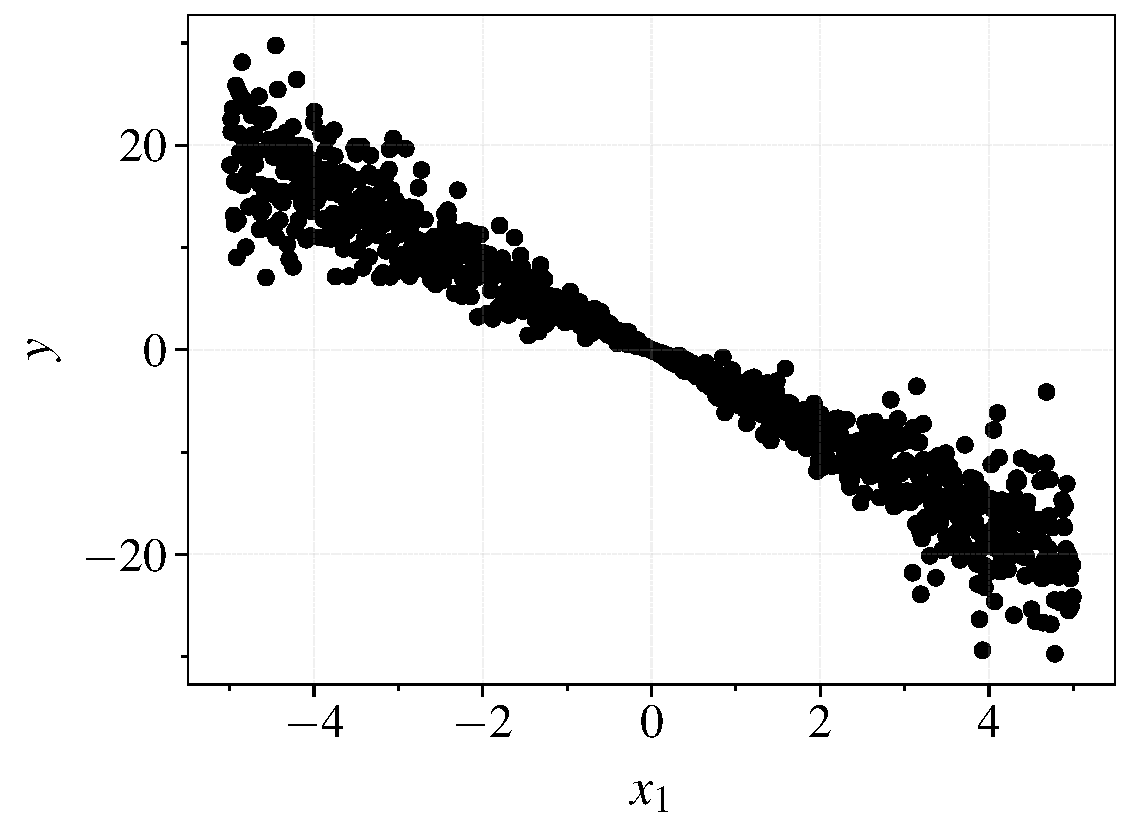
\includegraphics[width=\linewidth]{figures/example_x1.pdf} \\[\abovecaptionskip]
	  \small (a) Scatterplot of $y=f(x_1,x_2)$ and $x_1$.
	\end{tabular}

	\vspace{\floatsep}

	\begin{tabular}{@{}c@{}}
	  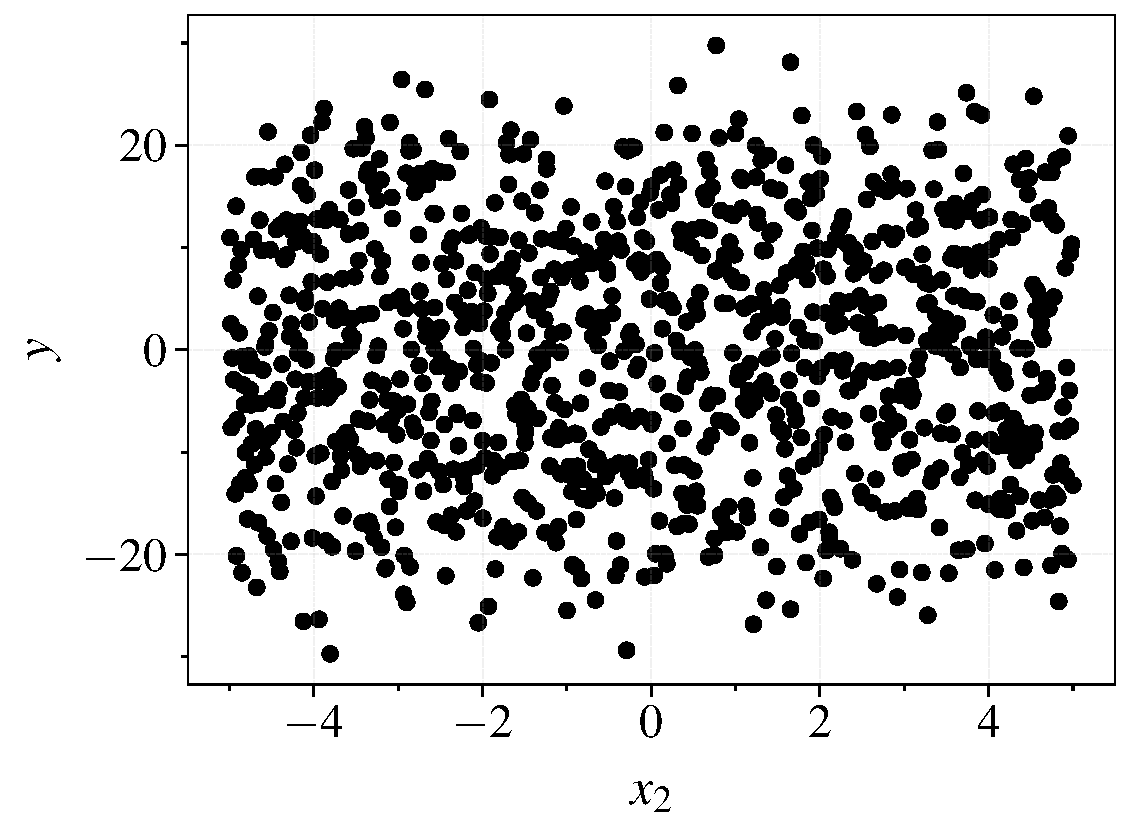
\includegraphics[width=\linewidth]{figures/example_x2.pdf} \\[\abovecaptionskip]
	  \small (b) Scatterplot of $y=f(x_1,x_2)$ and $x_2$.
	\end{tabular}

	\caption{Results of the evaluation of a black-box function $y=f(x_1,x_2)$ with $x_1,x_2 \in [-5,-5]$ using 1000 samples generated with Latin Hypercube sampling.
	Function $y$ shows strong dependence with $x_1$, but little or no dependence with $x_2$.}\label{fig:myfig}
\end{figure}

The dependence can be captured measuring the area described by the scatterplot, and comparing it to the box defined by $(\underline{y},\overline{y})\times(\underline{x_i},\overline{x_i})$.
If the measured area equals to the box, then it can be said that the output has no dependence on that input (as occurs for $x_2$ in Figure X).
If the measured area has a value of 0, it means that the output is determined by that input.
Then, any other degree of dependence will fall in between these two extreme cases (as in $x_1$ in Figure X).
It is important to note that the measurement of the area will be an approximation of the actual area, being a consequence of the sampling method or the subintervalization
if interval arithmetic is employed to solve the model functions.

The sensitivity index is calculated with the following formula:

\begin{equation}
	S_i = 1 - \frac{\sum_n^N(\underline{x_i},\overline{x_i})_n\times(\underline{y},\overline{y})_n}{(\underline{y},\overline{y})\times(\underline{x_i},\overline{x_i})}
\end{equation}

where $N$ is the total number of subintervals.
Therefore, $S_i$ is a sensitivity index ranging from 0 (i.e. $y$ is independent of $x_i$) to 1 (i.e. $y$ is determined by $x_i$).

The area can be calculated with two different methods depending on whether interval arithmetic was employed to calculate the functions or it was done though sampling.
In the case of interval arithmetic the calculation is straightforward as the subintervals can be recycled and the boxes described by these can be easily computed.
On the other hand, if sampling methods were chosen, then the area can be calculated employing an integration method similar to the trapezoidal rule: a step size is defined to
sweep through subintervals of $xi$ in the data, the minimum $\underline{y}$ and maximum $\overline{y}$ is returned for each subinterval, and the box is computed as usual.
The main drawback of the integration method is that a step size has to be defined manually, and the impact of this parameter on the proposed sensitivity analysis method has not
been studied yet.
However, the authors guess that since the method is similar to the trapezoidal rule, it should be possible to place error bounds on the accuracy of the sensitivity index.

Explain results using the example

%Figure with subboxes

Lastly, an important by-product of the proposed sensitivity index is that its calculation also entails the so called \textit{pinching} method [REF].
The \textit{pinching} sensitivity analysis calculates the reduction on the output uncertainty when the uncertainty of an input is reduced from the interval to a single value.
One drawback of this method is that a single value for each input interval has to be chosen (or several values within the interval, with the consequent
increase of computational cost).
However, the interval-based sensitivity index retrieves all the \textit{pinching} information possible for the given number of subintervals; so not only the
output dependence on the input is measured, but also how the input affects the output along its interval.
Figure 3 shows how reducing uncertainty in $x_2$ entails no reduction on the uncertainty of $y$, whilst reducing the uncertainty on $x_1$ has different consequences on the
uncertainty of $y$ depending on the value of $x_1$.
For example, the maximum output uncertainty reduction is obtained pinching for $x_1 = 0$.

%figures

\begin{enumerate}
	\item Introduce the area method (overview and illustrating example). [DONE]
	\item Use example and extreme cases to illustrate (e.g. perfect dependence = index of 1 = no area, independence = index of 0 = all area) [DONE]
	\item Show equation of the sensitivity index [DONE]
	\item Explain how it does with arithmetic (subintervalisation) [DONE]
	\item Explain how it does with sampling (integration similar to trapezoid rule) [DONE]
	\item Explain pinching. [DONE]
\end{enumerate}

\section{Application}

\begin{enumerate}
	\item Explain simple function (or physics based example?).
	\item Explain comparison with Sobol indices.
	\item Show results.
\end{enumerate}

\begin{enumerate}
	\item Explain Ishigami function
	\item Explain comparison with sobol indices (arguably the most common SA method)
	\item Show results.
\end{enumerate}

\section{Conclusion}

\begin{acknowledgement}
This section and its heading (unnumbered) should be in 9pt and come before the appendices and references.  Dedication and funding information may also be included here. 

\section*{References}

\bibliographystyle{chicago}
\bibliography{References}
\end{acknowledgement}


\end{document}




